\documentclass{article}
\usepackage[utf8]{inputenc}
\usepackage{geometry}
 \geometry{
 a4paper,
 total={170mm,257mm},
 left=20mm,
 top=20mm,
 }
 \usepackage{graphicx}
 \usepackage{titling}
 \usepackage{amsmath}
\usepackage[
    colorlinks=true,
    urlcolor=black
]{hyperref}
 \title{ Modeling Electro-Magnetic and Optical Sensors
}
\author{Sajjad Yami}
\date{November 2025}
 
\makeatletter
\def\@maketitle{%
  \newpage
  \null
  \vskip 1em%
  \begin{center}%
  \let \footnote \thanks
    {\LARGE \@title \par}%
    \vskip 1em%
    %{\large \@date}%
  \end{center}%
  \par
  \vskip 1em}
\makeatother

\usepackage{lipsum}  
\usepackage{cmbright}

\begin{document}

\maketitle

\noindent\begin{tabular}{@{}ll}
    Writer & \theauthor\\
     Adviser &  Mr. Baleghi\\
     Affiliation & \href{https://taha.ai/}{taha.ai} \\
     date & \thedate
\end{tabular}

\vspace{1em}
\hrule
\vspace{1em}

\section{Working Principles}
Electromagnetic and optical sensors are both widely used in our world. Here in this section, we briefly review how they work and what they measure.

\subsection{Magnetic Sensors}
Magnetic sensors convert the change in the magnetic field into an electric field. These sensors have a good tolerance to high vibration and environmental parameters. The output of the magnetic sensors is used to monitor the direction, location, revolution, angle, distance, speed, position, and the presence of electric current.
Any type of magnetic sensor works with the Earth's magnetic field. When an iron object approaches a magnetic sensor, it induces a magnetic field through the coil. This change generates the voltage at the terminals of the coil. This phenomenon is governed by Lenz’s law, which states: The current induced in a circuit due to a change in a magnetic field is directed to oppose the change in flux and to exert a mechanical force that opposes the motion.
\begin{figure}[htbp]
    \centering
    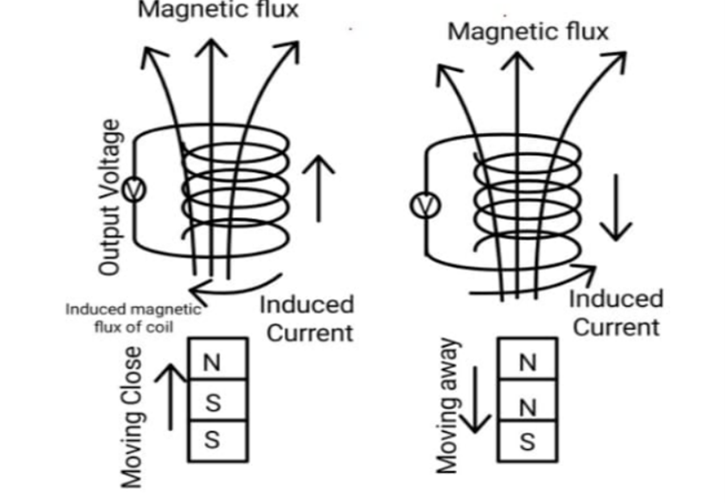
\includegraphics[width=0.5\linewidth]{images/lenz.png}
    \caption{Lenz's law}
    \label{fig:lenz's law}
\end{figure}

The most used magnetic sensor is the Hall effect magnetic sensor. The Hall effect is the production of a voltage (known as the Hall voltage) across an electrical conductor when a magnetic field is applied perpendicular to both the current flowing through the conductor and the resulting voltage. You can see a demonstration of how the Hall effect could detect a magnetic field in figure \ref{fig: Hall-effect}.
\begin{figure}[htbp]
    \centering
    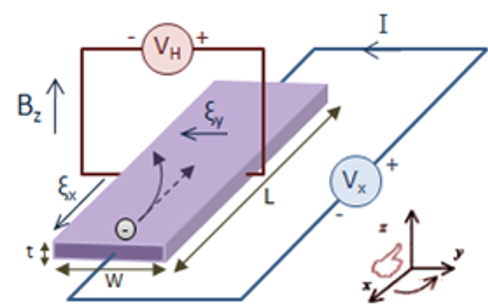
\includegraphics[width=0.5\linewidth]{images/Hall-effect .png}
    \caption{Hall effect}
    \label{fig: Hall-effect}
\end{figure}

There are two main categories in EM sensors: Active sensors and Passive sensors. Active sensors (like radar) transmit their own energy and receive the reflected signal back. For passive sensors (like cameras, radiometers, or infrared sensors), the concept is different. These sensors don't transmit anything. They just receive naturally available energy (reflected sunlight, thermal emissions, etc.).
\subsection{Optical Sensors}
Optical sensors' design is based on the Wheatstone bridge circuit. It has 4 resistors, 3 of which are known and 1 is unknown. By comparison, the ratio between these resistors, we can find the unknown. Optical sensors do the same with photodetectors. When the light is deflected, each sensor captures a different intensity of light. This information can be used for finding a position or detecting it.

Optical sensors can detect the location or presence of an object by emitting and receiving a beam of light. When the beam of light hits the object, it can pass through it or reflect from it.

We should choose our optical sensors according to our desires. As an example, for a transparent object, we need a more accurate device for the detection of the deflection of the beam. And for an object that has a texture on its surface, we need to capture the reflected beam and use the intensity and angle of the reflection to study the characteristics of the surface.

There are two important categories of optical sensors: imaging sensors and non-imaging sensors.
Imaging sensors are the sensors that capture spatial information to form an image. They tell you WHERE light is coming from in 2D space. This type of sensor can measure angles by triangulation from pixel positions.
Non-imaging sensors are the sensors that detect light intensity, position, or timing but do not form a complete spatial image. Some types of these sensors can give us some coordination, which could be used to find the angle of the object, like Position Sensitive Detectors (PSD, output is just 2 coordinates), but in contrast, photodiodes just give us a number, which is an intensity value. The difference between these two types of sensors is very important in the angle error parameter, which we will discuss in detail.

\section{Effective Range of EM and Optical Sensors}
The effective range of a sensor is the maximum distance or span over which the sensor can reliably detect, measure, or monitor a target or phenomenon while maintaining acceptable accuracy and performance. In this section, we discuss the parameters that could affect the effective range in both EM and optical sensors. 

In general, the effective range depends on how far the signal (or light) can travel before it falls below a usable threshold. Some parameters that affect the effective range in both EM and optical sensors are
\begin{itemize}
    \item Transmitted power $P_t$
    \item Receiver sensitivity $P_{r, \, min}$ (determines minimum detectable signal)
    \item Wavelength (Affects free-space path loss, higher frequency $\rightarrow$ higher loss)
    \item Atmospheric attenuation Absorption/scattering by air, fog, dust, or water vapor (especially for optical).
    \item Terrain and elevation (Line of sight (LOS) and diffraction around obstacles)
    \item Antenna/Sensors gain $G_t$, $G_r$ (Higher gain $\rightarrow$ more directed energy $\rightarrow$ longer range)
    \item Target reflectivity
    \item Weather conditions
\end{itemize}

In the upcoming sections, we try to model these parameters for both EM and optical sensors' effective range. For EM sensors, we introduce two models, which are called the link budget model and the Radar Range Equation (RRE) model. The link budget model is used for passive sensors, and the RRE model is used for active sensors. For optical sensors, we can use the Beer-Lambert Law to determine the effective range.
\subsection{Effective Range of EM Sensors}
As we mentioned, we can use the link budget model to estimate the effective range of an passive EM sensor. It tells you how much of your transmitted signal power actually arrives at the receiver, after all the gains and losses along the way. In linear form, it can be written as
\begin{equation}
    P_r = P_t\, G_t\, G_r (\frac{\lambda}{4 \pi R})^2 \frac{1}{L}\, .
\end{equation}
In dB form, we can write it as
\begin{equation}
    P_r = P_t + G_t - L_p - L_s\, .
\end{equation}
Here, $L_p$ is path loss (How much signal power weakens with distance), and $L_s$ is system or other losses (Cable loss, polarization mismatch, atmosphere, etc.). We can use free space path loss (FSPL) to calculate $L_p$.
The signal spreads spherically as it travels outward from the antenna. At distance R, the power density is diluted over a sphere’s surface area 4$\pi R^2$. So
\begin{equation}
    L_p = (\frac{4 \pi R}{\lambda})^2\, .
\end{equation}
In dB form, we can write it as
\begin{equation}
    L_p = 20\, log_{10}(\frac{4 \pi R}{\lambda})\, .
\end{equation}
This is the most fundamental propagation loss. We can even add atmospheric loss by a term like 
\begin{equation}
    e^{-\alpha R}.
\end{equation}
Recall that there is a threshold for the sensors below which the sensors cannot detect the signal. We name this threshold $P_r\,, min$ and we can fine $R_{max}$ by solving $P_r(R_{max}) = P_{r\,, min}$.
 Now, consider both path loss and attenuation, then the link budget formula can be rewritten as
 \begin{equation}
     P_r = P_t\, G_t\, G_r (\frac{\lambda}{4 \pi R})^2 \frac{1}{L} e^{-\alpha R}.
     \label{effective-range-active}
 \end{equation}
 This method is called budgeting because, like a financial budget, you start with a certain amount (transmit power), then add gains and subtract losses to see how much is “left” at the end. 
 We should be aware of the link margin = $P_r$ – $P_{r, min}$. If it is positive, it is a reliable link, and if it is negative, the link will fail.

For the estimation of the effective range of an active EM sensor, we can use the RRE formula.
The key difference is that while active sensors have a two-way path (transmit and receive), passive sensors have a one-way path (receive only), which fundamentally changes the form of the equations—particularly how range affects signal strength ($\frac{1}{R^2}$ for passive vs. $\frac{1}{R^4}$ for active radar in the simplest case). Another major difference is that in the passive case, the characteristics of the object that we want to detect are very important. By considering these two major differences, we can find the effective range of the active sensors by
\begin{equation}
    R_{max}=\left(\frac{(P_tG^2\lambda^2\sigma)}{(4\pi)^3S_{min}}\right)^{\frac{1}{4}}.
\end{equation}
Here, $S_{min}$ is the minimum detectable signal and $\sigma$ is the radar cross section. Everything else is just like the link budget model.
Recall that this formula is under ideal free-space conditions. 
 \subsection{Effective Range of Optical Sensors}
 If waves propagated through air, we could use the Beer-Lambert law to determine the effective range of an optical sensor. It measures light intensity as a function of distance.
 \begin{equation}
     I = I_0 e^{-\beta R}.
 \end{equation}
 Here, I(d) is the intensity at distance d, $I_0$ is the initial transmitted intensity, and $\beta$ is the atmospheric attenuation coefficient. Now, the effective range can be calculated by
 \begin{equation}
     R_{eff} = \frac{1}{\beta}\, ln(\frac{I_0}{I_{min}}).
     \label{eq;Beer-Lambert}
 \end{equation}
 But we should be aware of the linear response of the sensor. Beyond this point, the signal may become non-linear, making measurements inaccurate. This parameter can provide us with the maximum value for calculating the effective range.

 \section{Angle Error of EM and Optical Sensors}
Angle error (or angular error) refers to the uncertainty or inaccuracy in determining the angular position of a target relative to the sensor. It's the difference between the true angle and the measured angle. In this section, we investigate the parameters that can affect angle error in both EM and optical sensors.
There are general factors that could affect our accuracy in finding the angle, such as
\begin{itemize}
    \item Signal properties like wavelength
    \item Aperture size (Larger aperture $\rightarrow$ smaller bandwidth $\rightarrow$ less angular error)
    \item SNR (Higher SNR $\rightarrow$ lower error)
    \item Sampling rate (Affects accuracy of correlation)
    \item Multipath (Reflected signals cause phase errors)
    \item Alignment and calibration
    \item Elevation/Terrain (Uneven surfaces cause refraction or diffraction)
\end{itemize}
The angular error directly translates into the cross-range positioning error at the target location through the relationship $\Delta x = R \times \sigma_\theta$, where R is the range to the target. Therefore, even small angular errors can result in significant positional uncertainties at long ranges.
In the upcoming work, we introduce an empirical model for angle error for both EM and optical sensors. 
\subsection{Angle Error of EM sensors}
An Empirical model for RMS angular error (in radians) can be:
\begin{equation}
    \sigma_\theta=\frac{\lambda}{2\pi D\times S N R^{0.5}}\, .
\end{equation}
Here, D is the aperture size, like Antenna aperture diameter. The term $\frac{\lambda}{D}$ is related to the diffraction-limited beam-width (approximately $\frac{\lambda}{D}$ radians), which represents the sensor's intrinsic angular resolution. The dependence on $\sqrt{SNR}$ indicates that angle estimation accuracy improves with signal quality.
This model is invalid when the multi-path error is significant.

For example, for a radar with D = 1 m, $\lambda$ = 0.03 m (X-band), and SNR = 20 dB (ratio of 100), the angular error is approximately $\sigma \approx 0.5$ milliradians. At a range of 10 km, this corresponds to a cross-range error of about 5 meters.

\subsection{Angle Error of Optical Sensors}
In optical sensors, there is a subtlety. As we mentioned earlier, there are two major categories of optical sensors: imaging and non-imaging sensors. Each of these types has its own method to find the angle error.

Imaging sensors can provide coordinate data. The raw output of these sensors is pixel coordinates $(i, j)$. These coordinates could be transformed into x and y coordinates according to a reference.
\begin{align}
    x_{image} = pixel_{column} \times pixel_{pitch},\, \\
    y_{image} = pixel_{row} \times pixel_{pitch}.
\end{align}
Now, from this data, we can find the angle of the object. It is obvious from the formula that in imaging sensors, the angle error depends on the resolution of the sensor.
In imaging sensors, we should at least consider two major parameters that could affect the angle error: 1-Diffraction limit, 2-Sampling limit.

Diffraction limit comes from the physical blur from the wave nature of light. And the sampling limit is how finely you can sample the image.
The Diffraction-limited could be calculated by the formula
\begin{equation}
    \sigma_{\theta}^{diff} = 1.22 \frac{\lambda}{D}.
\end{equation}
Here, D is the aperture size and $\lambda$ is the wavelength.
This formula cannot be applied when sensors have larger errors than the diffraction limit, detector noise dominates, or non-imaging sensors are used.

The detector sampling limit comes from pixel pitch limitation. This quantity could be calculated by the formula
\begin{equation}
    \sigma_{\theta}^{smpl} = \frac{d}{f} \frac{1}{\sqrt{SNR}}.
\end{equation}
Here, d is the pixel pitch (physical size of one pixel) and f is the focal length.
We can choose the bigger error as our main error, or we can compute the RMS.
\begin{equation}
    \sigma_{\theta}^{tot} = \sqrt{\sigma_{diff}^2 + \sigma_{smpl}^2 + \sigma_{others}^2 }
\end{equation}

In non-imaging sensors, to have coordinate values, we can use position-sensitive detectors (PSD, output is just two coordinates), or we can make a setup to find the angle of the object. For example, consider photodiodes. These sensors just give a value (intensity) and don't provide any coordinate value. But by a setup, we could extract the coordinate value from the intensity. In this case, consider an arc of photodiodes. We could find the direction of the light source by finding the photodiode that receives the most light and reports the biggest intensity value. And compare the location of the photodiode with respect to a reference.
\begin{figure}
    \centering
    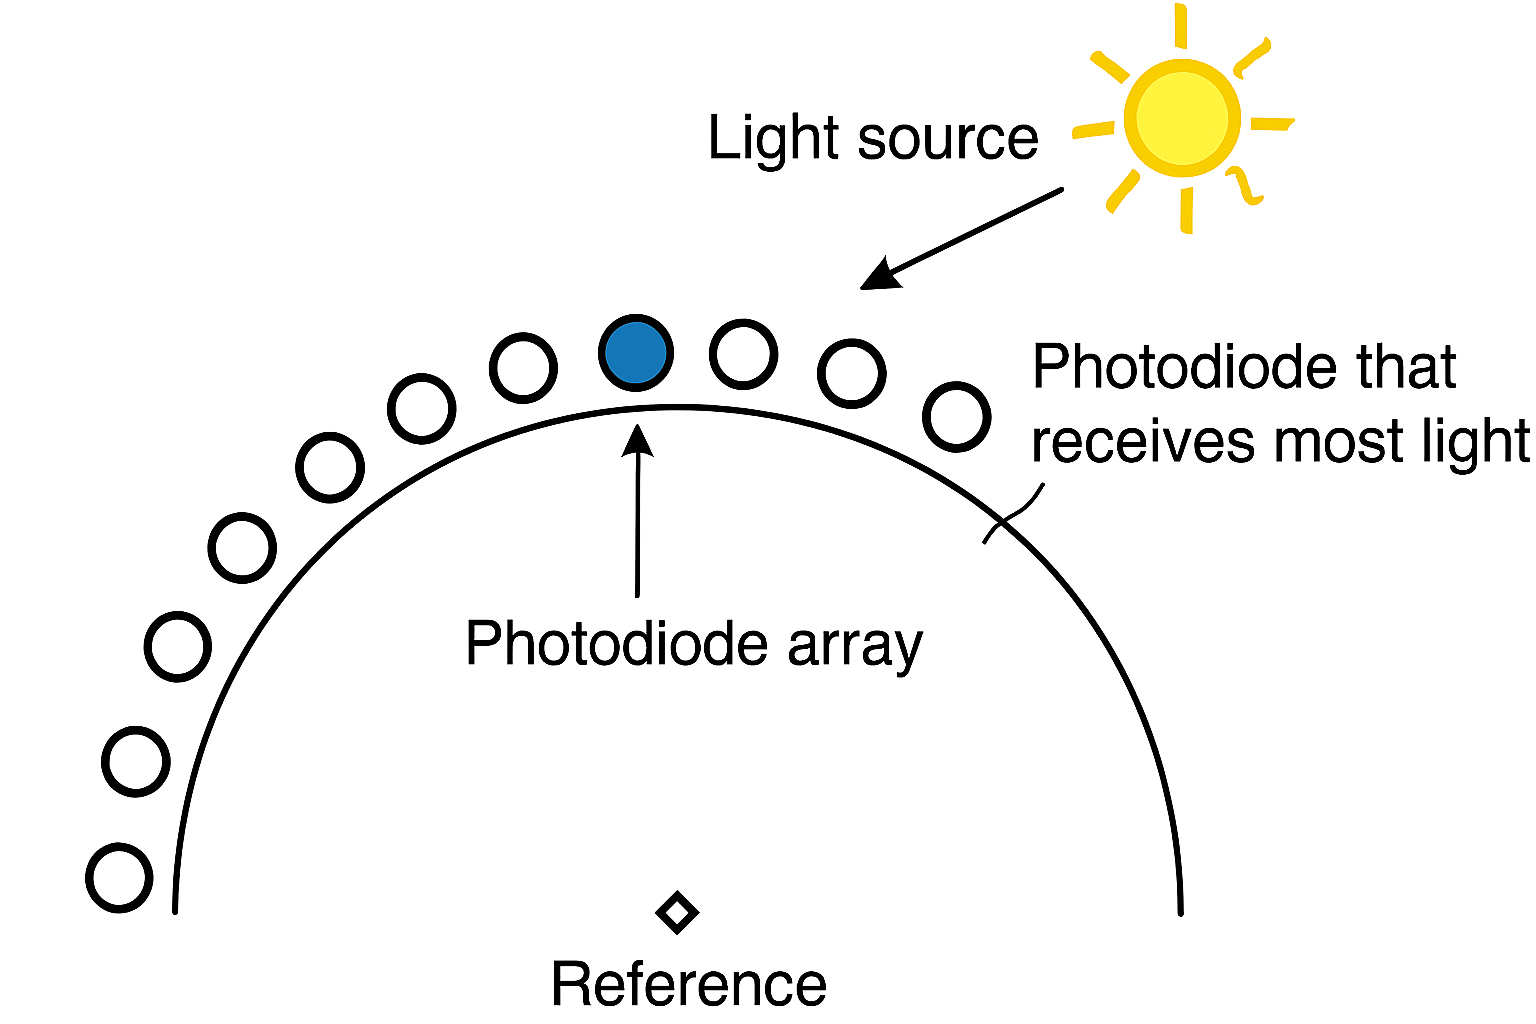
\includegraphics[width=0.5\linewidth]{images/photodiode.png}
    \caption{illustration of the photodiodes setup that could find the angle}
    \label{photodiodes}
\end{figure}
So, in non-imaging sensors, there is no unique formula. It highly depends on the sensors whether they can provide coordinate values or not. If they can't provide our angle error depends on our setup. 

For Example, we can use PSD. A PSD sensor, or Position Sensitive Detector, is an optical sensor that determines the position of a light spot on its surface.
A PSD provides a value that is our object's position. Then we could find the angle of the object by $\theta = arctan(\frac{X}{f})$. f is the focal length, and $\theta$ becomes the incident angle. So, the angle error could be written 
\begin{equation}
    \sigma_{\theta} = \frac{1}{f} \sigma_X\, .
\end{equation}
 $\sigma_X$ is the position measurement error of the PSD, and it depends on
 \begin{itemize}
     \item Position resolution $\sigma_X^{pos}$
     \item Noise-limited error $\sigma_X^{noise}$
 \end{itemize}
 Position resolution is specified by the manufacturer.
 Noise-limited error could be calculated by
 \begin{equation}
     \sigma_X^{noise} = \frac{spot\, diameter}{\sqrt{SNR}}.
 \end{equation}
 The "spot diameter" of a Position-Sensitive Detector (PSD) refers to the size of the light spot projected onto its surface.
 Then, we could use RMS to calculate $\sigma_X^{tot}$ by
 \begin{equation}
     \sigma_X^{tot} = \sqrt{(\sigma_X^{noise})^2 + \sigma_X^{pos})^2}\, .
 \end{equation}
 \newpage
\section{Terrain Effect}
Terrain elevation (or topography) simply means how the ground height varies with position. So in flat areas, it remains almost constant, but in hilly or mountainous areas, it can change rapidly. We can show it by $h_{terrain}(x,y)$, which gives you the height of the ground above some reference.

Terrain elevation is important in sensor modeling because of its effect on:
\begin{itemize}
    \item Line of sight blocking (Hills or other things can block the direct path)
    \item Diffraction or scattering (mainly for EM sensors), this effect can cause angle error
    \item Multipath reflection, this effect can cause angle error too
\end{itemize}
Here we describe the terrain as a height profile along the path between the transmitter and the receiver $h_{terrain}(x)$. If transmitter and receiver are at heights $h_t$ and $h_r$ above the ground and terrain elevation varies with distance x, then $h_{LOS}$ (LOS is line of sight) could be calculated by:
\begin{equation}
    h_{LOS}=h_t+\left(h_r-h_t\right)\frac{x}{R}\,.
    \label{eq:LOS}
\end{equation}
If $h_{terrain}(x) < h_{LOS}(x)$, then the signal path is clear and the effective range is determined by the \ref{effective-range-active} formula. And if $h_{terrain}(x) \ge h_{LOS}(x)$, then the effective range is limited to the position of the terrain. We can add diffraction models (like knife-edge diffraction) to estimate how much signal can bend around that obstacle, but it is more advanced.  
\begin{figure}[htbp]
    \centering
    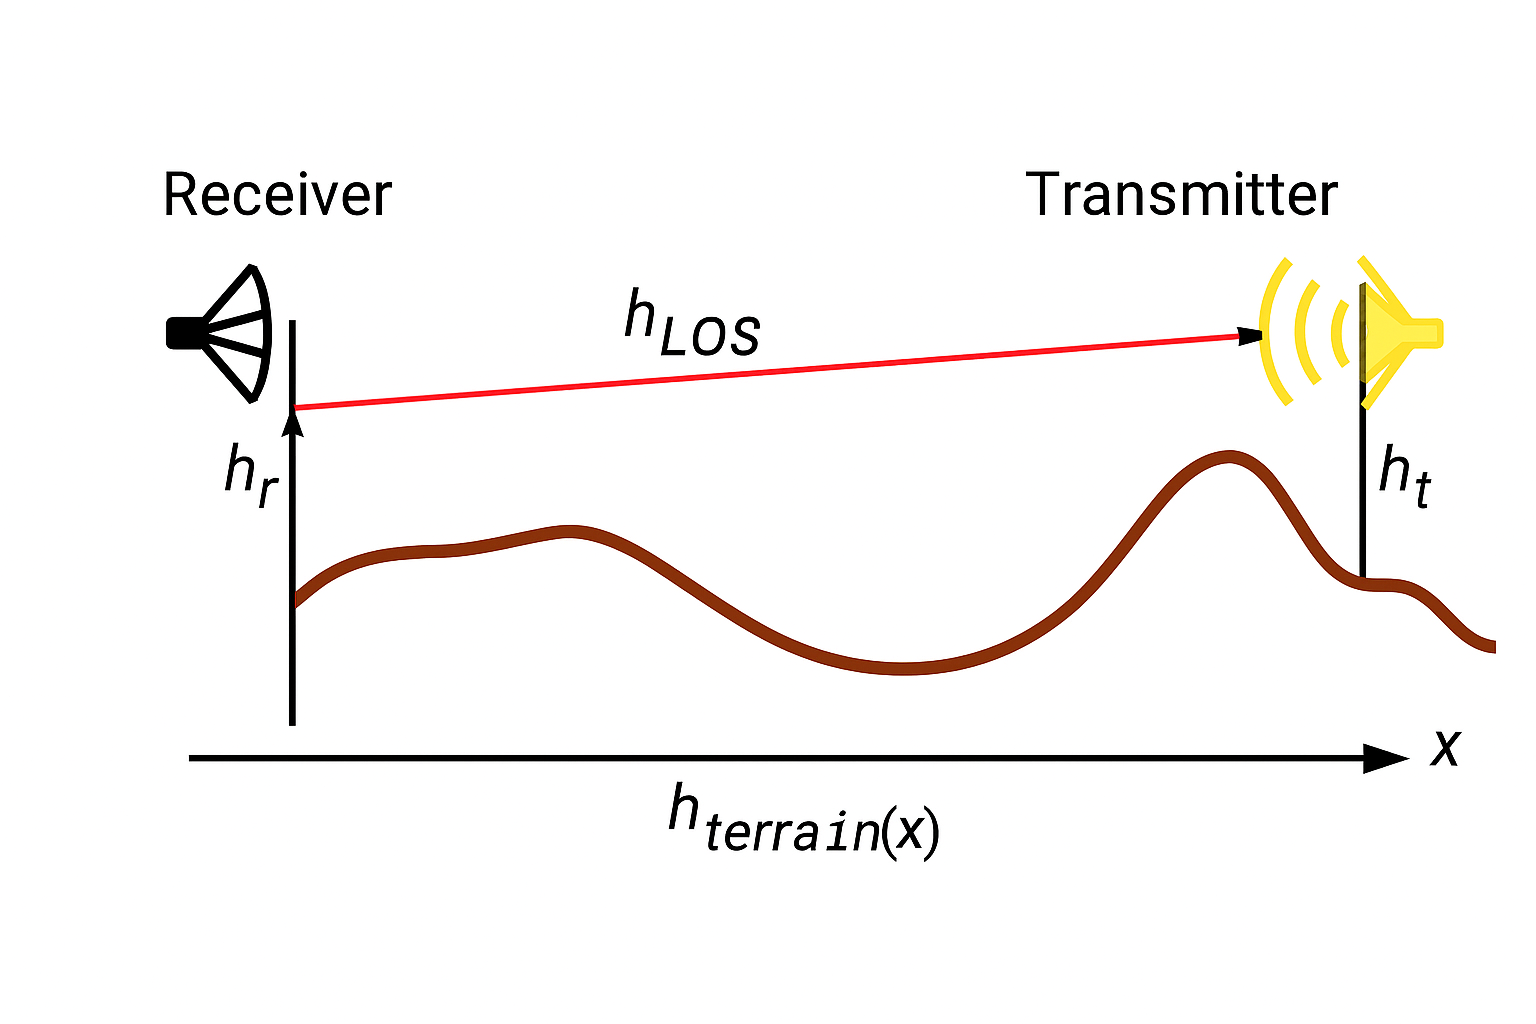
\includegraphics[width=0.5\linewidth]{images/terrain.png}
    \caption{Terrain effect}
    \label{fig:terrain-effect}
\end{figure}

\section{Elevation Effect}
The angle of elevation is the angle between the horizontal line of sight and an object that is above the horizontal line. To have a better understanding of what the elevation angle is, you could see the image below
\begin{figure}[htbp]
    \centering
    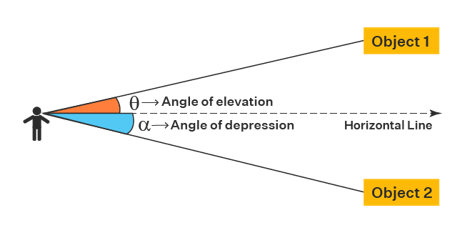
\includegraphics[width=0.5\linewidth]{images/elevation-angle.png}
    \caption{Elevation angle}
    \label{fig:placeholder}
\end{figure}

At low elevation, EM sensors are heavily impacted by terrain effects such as multi-path reflection and diffraction loss. In contrast, at high elevation, (for optical sensors) causes an increase in the total path length (air mass depth), increasing absorption and scattering loss.

If we have a receiver at a fixed height $(h_r)$ in a place with a terrain profile. We could measure the minimum angle for having a free line of sight.
\begin{align}
    \theta_{min}(x) = \frac{h_{terrain}(x) - h_{rec}}{x}, \\
    \theta_{LOS,\, min} = max\, \theta_{min}(x)\,.
\end{align}
In this angle, we have a clear path and less diffraction and scattering loss. Indeed, 
above $\theta_{LOS,\, min}$, the received signal strength and angle precision both improve. In RF link design, this angle threshold is exactly what’s used to check “clear Fresnel zone” conditions.

This formula is just applicable in short distances. In long-range, we should take into account Earth's curvature. We can modify $h_{terrain}$ to consider this parameter too.
\begin{equation}
    h_{eff} = h_{terrain} - \frac{x^2}{2R_e}\,.
    \label{eq:curve-earth}
\end{equation}
Where $R_e$ is Earth's radius.

For reliable LOS, we need not just a geometric path but clearance of the first Fresnel zone (the volume around the direct path that contributes significant energy).
The first Fresnel radius is
\begin{equation}
    r_F = \sqrt{\frac{\lambda d_1 d_2}{d_1 + d_2}}\, .
\end{equation}
Here, $d_1$ and $d_2$ are the distances from the transmitter (or source) to the point along the path where you’re evaluating the clearance and distance from that point to the receiver, respectively, and $\lambda$ is the wavelength.


If the terrain intrudes into that zone (typically $>$ 40 \% obstruction), you get noticeable diffraction loss even if the line barely clears it. If this happened, we could reduce the terrain effect by variation in elevation.

Besides these factors, we should consider atmospheric refraction. The EM path bends slightly downward due to the refractive gradient. To quantify this parameter, we need to see how much refraction causes in the effective Earth's radius.

\section{Modeling Assumption}
In developing the analytical models for electromagnetic (EM) and optical sensors, several simplifying assumptions were made to allow for tractable, first-order analysis. These assumptions are listed below along with their implications:
\begin{itemize}
    \item Free-Space Propagation – The link budget and range equations assume an unobstructed, homogeneous medium with no multipath or ground reflections. Real-world propagation introduces diffraction, refraction, and scattering effects that reduce range and increase angular error.
    \item Uniform Atmospheric Conditions – The attenuation coefficient ($\beta$) is assumed constant across the propagation path. In practice, humidity, temperature, aerosols, and wavelength-dependent scattering vary with time and altitude.
    \item Ideal Sensor Alignment – Transmitter and receiver are assumed perfectly aligned with stable mechanical mounting; misalignment or platform vibration introduces additional angular uncertainty.
    \item Reflections from terrain or structures are ignored except where terrain blocking is explicitly modeled.
    Flat-Earth Approximation (for short ranges) – Terrain and elevation calculations assume a locally flat Earth except where curvature correction is applied in Equation \ref{eq:curve-earth}.
    \item Linear Sensor Response – The optical and EM sensors are assumed to operate within their linear dynamic range; saturation or quantization effects are neglected.
\end{itemize}

\section{Implementation Plan}
In the implementation phase, we will try to get some parameters like:
\begin{itemize}
    \item Transmitted power
    \item Receiver sensitivity
    \item Wavelength or frequency
    \item attenuation
    \item Simple terrain profile
    \item Antenna/Sensors gain
    \item Aperture size
    \item others
\end{itemize}
Provide a model to calculate the effective range using equation \ref{effective-range-active} for EM and using equation \ref{eq;Beer-Lambert} for optical sensors.

Then calculate the angle error for EM sensors. For computing the angle error for optical sensors, we should know which type of optical sensors will be used, imaging or non-imaging. If they use a non-imaging sensor, which sensors would they be used with, PSD (that could provide coordinate value), or something like photodiodes (that could not provide coordinate value)?

Use a simple terrain profile and compute $h_{LOS}$ by equation \ref{eq:LOS}. Maybe try to compute the first Fresnel ellipsoid and then observe whether the terrain could affect the first ellipsoid or not.


\section{References}
We use these references for the proposal:
\begin{enumerate}
    \item Skolnik, M. I., Radar Handbook, 3rd Edition, McGraw-Hill, 2008.
    \item Hecht, E., Optics, 5th Edition, Pearson, 2016.
    \item IEEE Std 145-1993, IEEE Standard Definitions of Terms for Antennas.
\end{enumerate}
\end{document}
 